\documentclass{article}
\usepackage{amsmath}
\usepackage{graphicx}
\usepackage{hyperref}
\usepackage{listings}
\usepackage{xcolor}
\usepackage{tikz}
\usetikzlibrary{automata,positioning}

\definecolor{codegreen}{rgb}{0,0.6,0}
\definecolor{codegray}{rgb}{0.5,0.5,0.5}
\definecolor{codepurple}{rgb}{0.58,0,0.82}
\definecolor{backcolour}{rgb}{0.95,0.95,0.92}

\lstdefinestyle{mystyle}{
    backgroundcolor=\color{backcolour},
    commentstyle=\color{codegreen},
    keywordstyle=\color{magenta},
    numberstyle=\tiny\color{codegray},
    stringstyle=\color{codepurple},
    basicstyle=\ttfamily\footnotesize,
    breakatwhitespace=false,
    breaklines=true,
    captionpos=b,
    keepspaces=true,
    numbers=left,
    numbersep=5pt,
    showspaces=false,
    showstringspaces=false,
    showtabs=false,
    tabsize=2
}

\lstset{style=mystyle}

\title{Structured Output and Formal Languages: \\ Regex, Grammars, and Backus-Naur Form}
\author{AI Research Team}
\date{\today}

\begin{document}

\maketitle

\begin{abstract}
This article explores the relationship between structured output generation in Large Language Models (LLMs) and concepts from formal language theory, including regular expressions, context-free grammars, and the Backus-Naur Form (BNF). We examine how these classical concepts from computational linguistics have found new applications in controlling and constraining the output of modern language models, enabling more reliable and structured text generation for downstream applications.
\end{abstract}

\section{Introduction}

Structured output generation with Large Language Models (LLMs) represents a convergence of modern deep learning techniques with classical concepts from formal language theory. While LLMs are trained to generate natural language in a probabilistic manner, many applications require outputs that conform to specific syntactic structures or formats. This need has led to the adaptation of formal language concepts—such as regular expressions, context-free grammars, and the Backus-Naur Form—to constrain and guide LLM outputs.

These formal language concepts, which have been foundational in computer science and linguistics for decades, provide powerful tools for defining and constraining the structure of generated text. By leveraging these tools, developers can ensure that LLM outputs adhere to specific formats, making them more reliable for downstream processing and integration with other systems.

\section{Regular Expressions and LLMs}

\subsection{Overview of Regular Expressions}

Regular expressions (regex) are a sequence of characters that define a search pattern. They are commonly used for string matching and manipulation in various programming languages. Regular expressions are based on the theory of regular languages, which are the simplest class of formal languages in the Chomsky hierarchy.

A regular expression consists of:
\begin{itemize}
    \item Literal characters that match themselves
    \item Meta-characters with special meanings (e.g., *, +, ?, |)
    \item Character classes and quantifiers
    \item Grouping constructs
\end{itemize}

For example, the regex pattern `\\s*([Yy]es|[Nn]o|[Nn]ever|[Aa]lways)` matches strings that start with optional whitespace followed by one of the words "yes", "no", "never", or "always" (case-insensitive for the first letter).

\subsection{Regex-Based Constrained Generation}

In the context of LLMs, regular expressions can be used to constrain the model's output to follow specific patterns. This is particularly useful for ensuring that the generated text adheres to a predefined format or structure.

Libraries like Outlines implement regex-based constrained generation by:
\begin{enumerate}
    \item Converting the regex pattern into a finite state machine (FSM)
    \item Using the FSM to guide the token generation process
    \item Masking out tokens that would lead to invalid states in the FSM
    \item Renormalizing the probability distribution over the remaining valid tokens
\end{enumerate}

\begin{figure}
    \centering
    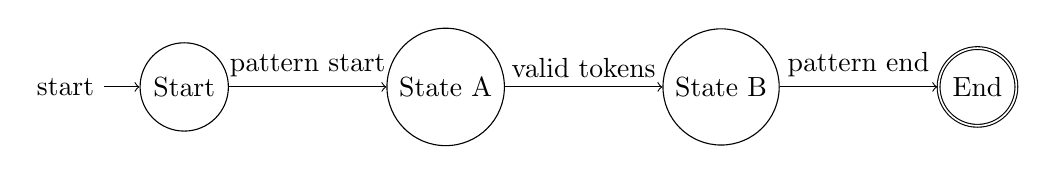
\begin{tikzpicture}[node distance=2cm, auto]
        \node[state, initial] (S) {Start};
        \node[state, right=of S] (A) {State A};
        \node[state, right=of A] (B) {State B};
        \node[state, right=of B, accepting] (E) {End};
        \path[->] (S) edge node {pattern start} (A);
        \path[->] (A) edge node {valid tokens} (B);
        \path[->] (B) edge node {pattern end} (E);
    \end{tikzpicture}
    \caption{Simplified finite state machine for regex-based generation}
    \label{fig:regex-fsm}
\end{figure}

This approach effectively transforms the unconstrained next-token prediction problem into a constrained generation problem where only tokens that maintain the validity of the regex pattern are considered.

\section{Context-Free Grammars and LLMs}

\subsection{Overview of Context-Free Grammars}

Context-free grammars (CFGs) are a formal grammar used to describe the syntax of programming languages, natural languages, and other structured formats. They are more expressive than regular expressions and can handle nested structures that regex cannot.

A context-free grammar consists of:
\begin{itemize}
    \item A set of terminal symbols (the actual characters in the language)
    \item A set of non-terminal symbols (abstractions that generate terminal symbols)
    \item A set of production rules that map non-terminals to sequences of terminals and non-terminals
    \item A start symbol (a designated non-terminal)
\end{itemize}

For example, a simple CFG for JSON-like objects might include rules like:
\begin{verbatim}
<object> ::= "{" <members> "}"
<members> ::= <pair> | <pair> "," <members>
<pair> ::= <string> ":" <value>
<value> ::= <string> | <number> | <object> | <array> | "true" | "false" | "null"
\end{verbatim}

\subsection{Grammar-Based Constrained Generation}

Grammar-based constrained generation extends the concept of regex-based generation to handle more complex structures. Instead of using a finite state machine, grammar-based generation typically uses parsing algorithms like CYK or Earley parsing to guide the generation process.

The key steps in grammar-based constrained generation are:
\begin{enumerate}
    \item Define a context-free grammar for the desired output format
    \item Track the parsing state during generation
    \item At each step, determine which tokens are valid continuations according to the grammar
    \item Mask out invalid tokens and renormalize the probability distribution
\end{enumerate}

This approach is particularly useful for generating structured outputs like JSON, XML, or programming code, where nested structures are common.

\section{Backus-Naur Form and LLMs}

\subsection{Overview of Backus-Naur Form}

Backus-Naur Form (BNF) is a notation technique for context-free grammars, often used to describe the syntax of programming languages, document formats, and communication protocols. It was developed by John Backus and Peter Naur in the late 1950s.

BNF uses a set of derivation rules written as:
\begin{verbatim}
<symbol> ::= expression
\end{verbatim}

where `<symbol>` is a non-terminal and `expression` consists of sequences of symbols and/or sequences separated by the vertical bar '|', indicating a choice.

Extended BNF (EBNF) adds additional notation for optional elements, repetition, and grouping, making it even more expressive.

\subsection{BNF-Based Constrained Generation}

BNF provides a formal way to specify the syntax of structured outputs, making it a natural choice for constraining LLM generation. By defining a BNF grammar for the desired output format, developers can ensure that the generated text adheres to the specified syntax.

The process of BNF-based constrained generation is similar to grammar-based generation:
\begin{enumerate}
    \item Define a BNF grammar for the desired output format
    \item Parse the grammar to create a representation that can guide the generation process
    \item During generation, track the current position in the grammar
    \item Constrain token selection to only those that are valid according to the grammar
\end{enumerate}

This approach is particularly useful for generating outputs in formats with well-defined syntaxes, such as programming languages or data exchange formats.

\section{Implementation in Modern Tools}

\subsection{Outlines: Finite State Machines for Structured Generation}

Outlines is a Python library that implements constrained text generation using finite state machines. It converts constraints (like regex patterns or grammars) into FSMs and uses them to guide the generation process.

The key innovation in Outlines is its efficient indexing approach that reformulates neural text generation using finite-state machines. This approach involves two main stages:

\begin{enumerate}
    \item \textbf{Preprocessing Step:} Converting a character-level deterministic finite automaton (DFA) into a token-level DFA that tests whether a token sequence decodes into a string matching the constraint.
    \item \textbf{Decoding Step:} Using the DFA to determine which tokens are allowed at each step, applying the corresponding mask to the next token probabilities, and updating the state of the DFA after each token is generated.
\end{enumerate}

\begin{lstlisting}[language=Python, caption=Using Outlines with regex constraints]
import outlines
import re

model = outlines.models.transformers("gpt2")

# Define a regex pattern for a simple email format
email_pattern = r"[a-zA-Z0-9._%+-]+@[a-zA-Z0-9.-]+\.[a-zA-Z]{2,}"

# Create a generator with the regex constraint
generator = outlines.generate.regex(model, email_pattern)

# Generate an email address
prompt = "Generate an email address: "
email = generator(prompt)
print(email)
\end{lstlisting}

\subsection{JSON Schema and Pydantic Models}

JSON Schema and Pydantic models provide another approach to structured output generation. These tools define the structure and validation rules for JSON data, which can be used to guide LLM output.

Libraries like LangChain and Outlines support JSON Schema and Pydantic models for structured output generation:

\begin{lstlisting}[language=Python, caption=Using Pydantic for structured output]
from pydantic import BaseModel, Field
from typing import List
import outlines

# Define a Pydantic model for the desired output structure
class Person(BaseModel):
    name: str
    age: int
    email: str
    skills: List[str] = Field(default_factory=list)

# Create a generator with the Pydantic model constraint
model = outlines.models.transformers("gpt2")
generator = outlines.generate.json(model, Person)

# Generate a person object
prompt = "Generate information for a software developer: "
person = generator(prompt)
print(person)
\end{lstlisting}

\section{Theoretical Connections and Practical Implications}

\subsection{Chomsky Hierarchy and LLM Constraints}

The Chomsky hierarchy classifies formal grammars into four types based on their expressive power:
\begin{enumerate}
    \item Type-0: Unrestricted grammars
    \item Type-1: Context-sensitive grammars
    \item Type-2: Context-free grammars
    \item Type-3: Regular grammars
\end{enumerate}

LLM constraint mechanisms typically operate at the level of Type-3 (regular expressions) or Type-2 (context-free grammars) in the Chomsky hierarchy. This is because these types of grammars are computationally tractable and can be efficiently implemented as constraints during the generation process.

The choice of constraint mechanism depends on the complexity of the desired output structure:
\begin{itemize}
    \item Regular expressions are sufficient for simple patterns without nested structures
    \item Context-free grammars are necessary for formats with nested structures (like JSON or programming languages)
    \item More complex constraints might require post-processing or additional validation
\end{itemize}

\subsection{Practical Implications for LLM Applications}

The integration of formal language concepts with LLMs has several practical implications:

\begin{itemize}
    \item \textbf{Improved Reliability:} By constraining outputs to follow specific formats, LLMs become more reliable for critical applications.
    \item \textbf{Reduced Post-Processing:} Structured outputs reduce the need for complex post-processing logic to extract information from free-form text.
    \item \textbf{Better Integration:} Structured outputs facilitate seamless integration with downstream systems that expect data in specific formats.
    \item \textbf{Enhanced User Experience:} Consistent, well-formatted outputs improve the user experience in applications like chatbots or code generation tools.
\end{itemize}

\section{Future Directions}

The integration of formal language concepts with LLMs is an evolving field with several promising directions for future research and development:

\begin{itemize}
    \item \textbf{More Expressive Constraints:} Developing constraint mechanisms that can handle more complex grammars while remaining computationally efficient.
    \item \textbf{Semantic Constraints:} Extending beyond syntactic constraints to include semantic constraints that ensure the generated content is not only well-formed but also meaningful and accurate.
    \item \textbf{Hybrid Approaches:} Combining different constraint mechanisms (e.g., regex for simple patterns and grammars for complex structures) to achieve the best balance of flexibility and control.
    \item \textbf{User-Friendly Interfaces:} Creating more intuitive interfaces for defining constraints, making these techniques accessible to a wider range of users.
\end{itemize}

\section{Conclusion}

The integration of formal language concepts with LLMs represents a powerful approach to structured output generation. By leveraging regular expressions, context-free grammars, and the Backus-Naur Form, developers can ensure that LLM outputs adhere to specific formats, making them more reliable for downstream processing and integration with other systems.

As LLMs continue to evolve and find applications in more domains, the importance of structured output generation will only increase. Understanding the theoretical foundations and practical implementations of these techniques will be essential for developers looking to build robust and reliable LLM-powered applications.

\section{References}

\begin{enumerate}
    \item Chomsky, N. (1956). Three models for the description of language. IRE Transactions on Information Theory, 2(3), 113-124.
    \item Hopcroft, J. E., Motwani, R., & Ullman, J. D. (2006). Introduction to Automata Theory, Languages, and Computation. Pearson Education.
    \item Liang, P., et al. (2024). Holistic Evaluation of Language Models. arXiv preprint arXiv:2211.09110.
    \item Outlines. (2024). Outlines: Structured Generation with LLMs. https://github.com/outlines-dev/outlines
    \item Tran-Thien, L. (2024). Outlines: Guided Generation with LLMs. https://outlines-dev.github.io/outlines/
    \item Willard, B., & Louf, J. (2023). Guided Generation: Constrained Decoding for LLMs. arXiv preprint arXiv:2307.09702.
\end{enumerate}

\end{document}
